\section{Use Case Diagrams}

This section outlines the use cases for the product. Standard UML notation is used. There are 4 elements, the actor who interacts with the system, the use cases, that are tasks that can be performed by the system, and lines that represent relationships between the actor and the system. The fourth element is the system or application itself, which is not viualized here, but which is made up of all the use cases in the given diagram. The lines that are marked "include" are used to show the relationship between use cases where one can be reached from the other. \cite{usecaseUML}


\begin{figure}[H]
  	\centering
	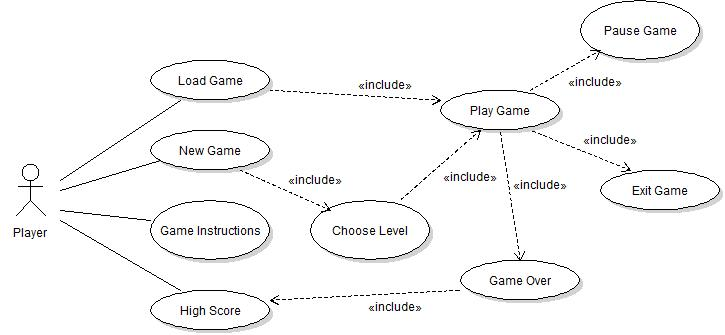
\includegraphics[width=\textwidth]{pictures/UCD_Game_Menu_After.jpg}
	\caption{Use Case Diagram of Game Menu}
\end{figure}

\begin{figure}[H]
  	\centering
	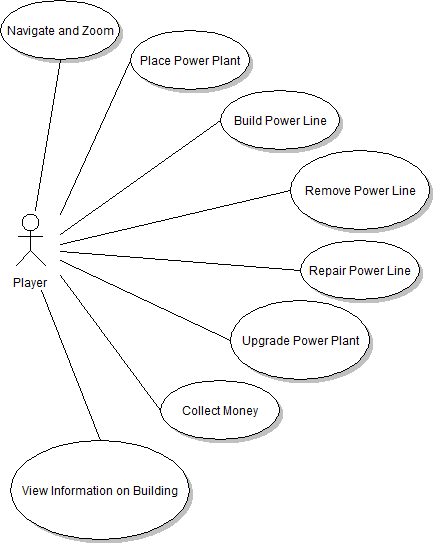
\includegraphics[width=\textwidth]{pictures/UCD_PlayGame.png}
	\caption{Use Case Diagram of Gameplay}
\end{figure}

